        % Chapter 1

\chapter{Summative Evaluation} % Main chapter title

\label{summativeevalchapter} % For referencing the chapter elsewhere, use \ref{Chapter1} 

\lhead{Chapter \ref{summativeevalchapter}. \emph{Summative Evaluation}} % This is for the header on each page - perhaps a shortened title

%----------------------------------------------------------------------------------------
\section{Recruitment of Participants}
With the help of one research assistant and her team (one female field worker who also became one of the adult subjects in the study), I managed to recruit a total of 14 adult participants (beneficiary users) through convenience sampling. By the ``researcher'', in the context of this chapter, I mean myself. In cases where I use ``we'' within text, it implies the researcher and research assistant's team collaborated in doing the work. The research assistant's team approached potential participants for the study at the beginning of  October 2015, and recruited participants from two townships in Cape Town, namely Langa (where the research assistant resided) and Athlone (where the field worker resided). The research assistant coordinated the process while the field worker assisted her. Out of 14 adults, Langa had five, while in Athlone there were nine. There was only one male out of 14 adult participants. It was easier to  recruit females than males, as females were more eager to participate than males; this resulted in a gender imbalance among adult participants.  The study in Chapter \ref{prototype2chapter} also showed this trend of gender imbalance, with more females present. The average age of these adult participants was 44.21 years, with a standard deviation (SD) of 9.99 years. The age range was between 26 and 60 years. The highest education level among adult participants was secondary school, while the lowest was the last grade of primary school. 

The research assistant's team notified adult participants before recruitment that one of the requirements to be part of the study was to have a family member, preferably a schoolgoing child, willing to be part of the study. Each adult participant we recruited elected/brought one of their children/grandchildren to act as their intermediary user. The two people, an adult and a child, formed one pair of users. As a result, we had 14 children in the study. Thirteen adult participants teamed up with their children, and the remaining one adult teamed up with her grandchild. Child participants had a mean age of 15.42 (with a standard deviations of 2.06 years), and the age range of child participants was between 12  and 20 years. There was a gender balance among intermediary participants. 

I visited the two research sites on separate occasions (days) to talk to all participants (adults and children). In these meetings, I gave out detailed information of what the study was about to both intermediary and beneficiary participants. I informed them about the different ways I would be collecting data. The data collection approaches included usage logs, questionnaires and interviews (see more details in section \ref{datacollect} -- Data Collection and Analysis). All the beneficiary participants signed informed consent forms agreeing to be part of the study. Since all intermediaries were under 21 years of age (the legal age for giving consent in South Africa is 21 and above), they signed assent forms which were also signed by their respective parents/guardians who were part of the study.

I allocated one day for training all intermediary participants how to use the Family Wellness app. I conducted training in Athlone (one of the research sites), and the research assistant and her team organized transport for children from Langa (the second site) to be able to attend this meeting. The reason we brought the children together was, firstly, to let them become acquainted with each other (this would be instrumental in gamification). Secondly, it was a good idea to train all intermediary participants at once so that they could start using the Family Wellness app immediately after the training. During the training, each intermediary participant/user received a user manual. After the training, I assigned one Android phone (Samsung GT-S5300) to each pair of participants; children collected these phones on behalf of their parent or grandparent. In each phone, I had installed two native apps on each phone (same apps used in Chapter \ref{prototype2chapter}): the pedometer app and the main `Family Wellness app. The Family Wellness app loaded all its content from a web application, which I hosted at the University of Cape Town. There were two versions of the web app, and I have described the details of these two versions in the Experiment Design section (\ref{exp_design}) below. Each beneficiary participant had to carry the  pair's assigned phone in order for the pedometer app to count their footsteps. Participants had six weeks to use the two apps (main app and pedometer).~Each pair of participants provided the phone number of the SIM card that would be inserted into their given Android phone. I allocated 1.3GB of data to each SIM card, and each beneficiary participant was given a total of ZAR240 ($\approx$ US\$20) for the duration of the study. This amount covered compensation for participants' transportation and time spent on data collection activities such as questionnaires and interviews. The details of the experiment are outlined in the next section. 

\section{Experiment Design}\label{exp_design}
The research objective was to evaluate the effectiveness of gamification in promoting intermediated use in the context of personal health informatics. Therefore, the experiments entailed comparisons between an app that was not gamified and a gamified app. The non-gamified app (the logbook app) was simply a diary/journal part of the prototype described in Chapter \ref{prototype2chapter} -- it enabled pairs of participants to track both the nutritional components of the meals a beneficiary participant consumed and the footsteps of the beneficiary member. The second version of the application was an extension of the logbook; it included all the features of the logbook with the addition of a rewards/gamified subsystem. The details of the gamified subsystem have also been provided in the previous chapter (Chapter \ref{prototype2chapter}). I carried out the experiments from mid-October 2015 to the end of November 2015.

I opted to use the ``within-group'' approach for the experiment design. In this approach there are no fixed control/intervention groups, as the same group of subjects have a chance to experience both control and intervention conditions. The rationale for choosing this design approach was that it reduces interference from confounding factors. The second benefit is that it reduces the cost of recruitment, as the same group is observed in both control and intervention conditions. This approach could also be of benefit in ICTD: recruitment of participants is one of the daunting tasks in ICTD studies~\citep{anokwa2009stories,ramachandran2010research} and this may compromise the rigour of such studies~\citep{ramachandran2010research}. The within-group approach offers benefits in terms of increasing the power of a study by using only half the number of subjects/participants that would have been required in a typical control/intervention study.

I created two experimental conditions one referred to as the logbook condition and one referred to as the gamification condition, and used the same group of subjects for both conditions. There is a caveat in using this approach: the learning effect could affect the rigour of the findings  if all participants start together in one experimental condition and thereafter switch to the other experimental condition. The learning effect would favour any experimental condition that comes first (predecessor), and disadvantage the one that comes last (successor). I dealt with this particular issue by creating experimental sequences, as highlighted in the next paragraph. 

I divided pairs of participants into two groups, the difference being the order in which experimental conditions started and finished.  I referred to each of these modes of starting and finishing as an experimental sequence. Therefore, both groups had a unique experimental sequence. I labelled these two groups ``LG'' and ``GL''.  In the LG group, pairs of participants started with the logbook condition and later switched to the gamification condition. In the GL group, pairs of participants started with the gamification condition and later switched to the logbook condition. I designed the switching of experimental conditions to happen at the midpoint of the experiment. These experimental sequences prevented the learning effect from affecting individual experimental conditions. The objective was to cancel out the learning effect, as each experimental condition was present before midpoint and after midpoint. One drawback of the within-group approach is that it makes the duration of experiments much longer, and this can be tiresome for research participants. However, this was an added advantage for this particular research, since the study was trying to understand any differences in sustained usage of a system using logbook and a system using gamification.

I randomly selected and assigned seven pairs of participants to the LG group, while the remaining seven pairs went to the GL group. Initially the plan was to have the time spent on each experimental condition be three weeks, but phase 1 had extended beyond its allocated block of three weeks up to the fourth week, as pairs of participants were not available for midpoint assessments at the end of the third week. Therefore, I carried out the midpoint assessment at the end of the fourth week. After the assessment, pairs that were using the gamified app switched to using the logbook app, and vice versa. It was not feasible to extend phase 2 to four weeks as in phase 1, because it was approaching December when most people travel for holidays; gathering participants during that time would have been impractical. This shortened the duration of phase 2 to two weeks. These kinds of eventualities are common in field research within the ICTD context. Researchers have argued that even though eventualities may appear to affect the rigour of research, such compromises offer benefits as they tend to preserve contextual interactions which are key to facilitating an intervention~\citep{anokwa2009stories,ramachandran2010research}. Through the course of doing the series of studies reported on in previous chapters up to the current reported study, not everything went according to plan, and compromises and constant negotiations had to be made; these contextual aspects were vital in making this intervention/research a success. Compromises on the rigour of the methods, and how it offered benefits in terms of preserving contextual factors, played an important role in this study. Examples of negotiations were on issues to do with recruitment of participants, and location (meeting points for interviews) and the availability of participants -- interaction between space and time. The aim of this study was not to make any generalization based on statistical tests, but rather to garner insights on human factors on intermediated use when utilizing gamification.  As a result, the takeaways and contribution made by this study are still valid when considering the arising need to understand and preserve the social relations that were crucial in the execution of this field work.
\section{Data Collection and Analysis}\label{datacollect}
I carried out data collection through a triangulation of the application's usage logs, questionnaires and interviews. Questionnaires and usage logs resulted in the generation of quantitative data, while interviews yielded qualitative data. Triangulation of different methods is important when doing research in ICTD, as it strengthens the reliability of the findings~\citep{burrell2009constitutes}.

I analysed quantitative data using both descriptive and inference statistics. Before each inferential statistical test, I tested data points to see if they followed normal distribution. The test that I applied to check for normality was the \emph{Shapiro-Wilk Normality Test}\footnote{http://sdittami.altervista.org/shapirotest/ShapiroTest.html}. I have outlined my reasons for choosing specific statistical tests below.
\begin{enumerate}[label=(\alph*)]
\item  Part of the quantitative data consisted of sets of data with paired samples (two dependent samples) used for analysis. On deciding what statistical test to use, the first step was to test the normality of the difference between repeated measures of each data point. If there was no normality, I would apply a log transformation on the original data, and repeat the normality test. For cases where the data assumed normality, I used parametric tests such as the student-t test with repeated measures. All the sets of paired samples achieved normality on either the original data or transformed data; as a result, non-parametric tests where never used in cases of all sets of two dependent samples.
\item Quantitative data also consisted of sets of data with three dependent samples. In the first step, I paired each sample to one sample from the same set. This process created three pairwise samples. Then  I used the same procedure to check for normality in two dependent samples. In all cases where there were three dependent samples, there was normality on the original data; hence the data did not need any transformation. As a result I ended up using one-way analysis of variance (ANOVA) with repeated measures in all cases where there were three dependent samples.  
\item The third part of the quantitative data sets consisted of two independent samples. I did the normality test on each independent sample. In the absence of a normal distribution in any of the two independent samples, a log transformation was applied. In some cases, data followed normal distribution. In such cases, I used the student-t test with no repeated measures. There was one case of two independent samples that did not adhere to the requirement of normal distribution on either original data or transformed data. In that case, I resorted to using the Mann-Whitney U test -- a non-parametric test\footnote{Mann-Whitney test, a non-parametric test for independent samples}. 
\end{enumerate}
The next subsections provide details of the three data collection methods used in this study.
\subsection{Family Wellness App Logs}
\subsubsection{Generation of Usage Logs}
The web application captured usage logs on the client (user) side through JavaScript events. The app generated events when users touched/clicked links that loaded features/functionality on the app. Asynchronous JavaScript (AJAX) transferred all events to the server for storage on a database, after wrapping them into JSON (JavaScript Object Notation) format. Each object mapped a pair's identity to events in order to know to whom events belonged. Figure \ref{figure:events_logs} shows the logical organization for capturing, transferring and storing events.
\begin{figure}[htbp]
  \centering
    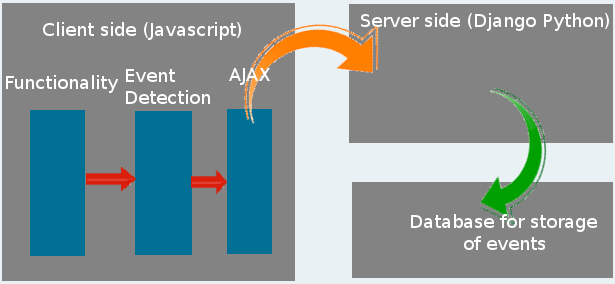
\includegraphics[width=0.6\textwidth]{Figures/events_capture.png}
    \rule{35em}{0.5pt}
  \caption{Generation of usage logs.}
  \label{figure:events_logs}
\end{figure}
Before sending out events, the client application stored them temporarily   until the user moved from one functionality to the other. Then AJAX would send out past events that the client program had already stored in its variables. Due to this delay, the server program was not recording events in real time. This approach of delaying until the user accessed the next feature was intentional in order to minimize the frequency of data transfers between clients and server. This delay did not affect the ability to understand the usage behaviour pattern. 

I chose not to capture the client's clock time on the client side during the capturing of events, because recording the phone's time on the client side had its limitations. There were periods during which the dates on the experimental phones were not correct. I had learned in previous studies (Chapters \ref{prototype1chapter} and \ref{prototype2chapter}) that participants had a tendency of removing SIM cards from their phones, and this would require removing the batteries. After removal of its battery, a phone would lose its clock time. If a user then tried to access the app immediately, time recordings would be incorrect; for instance, the Android phones used for the experiments would set date and time to the default one from the manufacturer. I noticed this pattern by looking at the logs from a pedometer: there were times when the pedometer reported a few incorrect time readings. I confirmed this behaviour of changing SIM cards during interviews reported on in Chapters \ref{prototype1chapter} and \ref{prototype2chapter}. Because of the above stated reasons, I made a decision to capture the time of events on the server side. 

Once events arrived on the server side, the server program (written in Python) would attach on arrival time and store those events in a database. Therefore, the database kept information such as when there was user activity on the app, which pair was accessing the app at that time, and what functionality/feature a pair accessed. The system also categorized events into their respective experimental conditions.  
\subsubsection{Analysis of Usage Logs}\label{log_analysis}
Through the analysis of events that the app was able to capture, I was able to synthesize usage into two useful dimensions: (1) the number of usage sessions of each pair of participants; and (2) the number of views of certain features by each pair of participants, which I will refer to as the ``number of impressions''.

I defined a new session as starting when user activity on the app was detected after an absence of any activity by that particular user/pair in the past one hour or more. The term ``impressions'' is commonly used in social network platforms (e.g. Instagram) to describe views on status updates by userz (things posted by users e.g. text, photos, etc.). In this context, I define impressions as the number of times a certain feature was viewed by a pair. If multiple clicks by one user/pair on one feature happened within an interval of less than one minute, they were grouped as a single impression. If clicks on the same feature differed by a minute or more, I then considered the current click to be a new impression while the previous click belonged to the previous impression. If the time difference between clicks on the same feature was beyond one minute, then it was assumed that the user had gone away or moved to a different feature and was coming back to this feature for another series of clicks. The purpose of computing a pair's total impressions on each feature was to understand where users of the app were likely to go among the many options of gamification features, namely leaderboard (score board), score badge, botanical garden and fish tank (fish aquarium). 
 
I conducted two major analyses of usage logs by using data on number of impressions and sessions. 
\subsubsection*{Comparison of Usage Sessions Between Logbook and Gamification.}
This particular analysis was twofold.
\begin{enumerate}[label=(\alph*)]
\item \textbf{Comparison of Daily Total Sessions Between Logbook and Gamification}
\end{enumerate}
In the first part of this comparison, I obtained the daily total number of sessions in each experimental condition, through adding sessions from all users in an experimental condition. I repeated this process for all 41 days of running the experiment, using the format of Table \ref{table:totaldailysessions}. As the result there were 41 data points. I then compared daily total sessions of logbook and gamification. I treated each experimental condition as an independent variable. I also treated the total number of sessions from all users in a particular experimental condition as a dependent variable.    

\begin{table}[h!]
  \begin{center}
    \caption{An example of total daily sessions from each experimental condition.}
    \label{table:totaldailysessions}
	\begin{tabular}{|l|l|p{6cm}|}
		\hline
		Day&Daily total of logbook sessions&Daily total of gamification sessions\\
		\hline
		Day 1&X&Y\\
		\hline
		Day 2&......&...... \\
		\hline
		.&.&. \\ 
		.&.&. \\   
		 && \\  
		.&.&. \\ 
		.&.&. \\ 
		\hline
       	Day 41&U&V \\
		\hline
	\end{tabular}
  \end{center}
\end{table}

The statistical test that I applied to do the comparison was the Mann-Whitney U Test. I highlighted at the beginning of this section (\ref{datacollect}) how arrived at the decision of choosing one among different tests in each case of inferential statistical analysis. 
\begin{enumerate}[label=(\alph*)]
\setcounter{enumi}{1}
\item \textbf{Comparison of Sessions Between Logbook and Gamification in Each Pair}
\end{enumerate}
I conducted the second comparison between sessions in logbook and gamification at the level of individual pairs of participants. In this comparison, I was looking at how each pair performed in logbook and gamification (i.e. repeated measures for usage during logbook and usage during gamification by the same pair of users). The number of weeks spent on the experiment prior to the midpoint assessment (four weeks) was not the same as the number of weeks spent on the experiment after the midpoint assessment (two weeks). Therefore, it was not fair to compare between an experimental condition that was available for four weeks and an experimental condition that was available for only 2 weeks. For instance, if a pair had started with logbook, they then spent four weeks in logbook and two weeks in gamification. The reverse applies for a pair that started with gamification. In order to make the comparison of the number sessions by the same pair of participants in the two experimental conditions fair, I opted to use a relative (normalized) number of sessions  as a unit of measurement. The formula I used for the normalized number of sessions is as shown below,
\begin{mdframed}[style=MyFrame]
$$T_{mj}=S_{mj}/D_{mj}$$
\end{mdframed}
\textbf{where}:

$T_{mj}$ is the number of sessions per day for a pair $m$ in experimental condition $j$,


 $S_{mj}$ is the total number of sessions for a pair $m$ in experimental condition $j$, and

$D_{mj}$ is the total number days on which pair $m$ could access experimental condition $j$ (27 days $\approx four$ weeks if the experimental condition started before midpoint, and 14 days = two weeks if the experimental condition started after midpoint).
%\noindent

I formulated a hypothesis with the aim of understanding the difference in usage sessions for the same pair of participants, when in logbook and when in gamification.

\begin{enumerate}
   \item{Hypothesis 1}
      \begin{itemize}
       \item{H\SB{0}}: There is no difference in the normalized number of sessions of a logbook app and a gamified app
       \item{H\SB{A}}: There is a difference in the normalized number of sessions of a logbook app and a gamified app
      \end{itemize}
   \end{enumerate}
   
I made a decision to exclude four pairs in testing the aforementioned hypothesis. These were pairs that faced hurdles when utilizing the app as a result of technical glitches. Technical glitches affected their performance in terms of usage sessions. Table \ref{table:usageproblems} provides a list of excluded pairs. 

\begin{table}[h!]
  \begin{center}
    \caption{Excluded pairs as the result of technical glitches.}
    \label{table:usageproblems}
	\begin{tabular}{|l|l|l|p{6cm}|}
		\hline
		&Pair&Group&Problem\\
		\hline
		1&Pair-A&GL-sequence &App failed to load due to poor Internet connectivity and malfunctioning of the phone.\\
		\hline
		2&Pair-B&GL-sequence&This pair didn't have data bundles due to misallocation. \\
		\hline
		3&Pair-C & LG-sequence& Their pedometer didn't transmit steps throughout the duration of the study.\\
		\hline
		4&Pair-D & LG-sequence& Pedometer worked for a while before it stopped transmission of data.\\
	\hline
	\end{tabular}
  \end{center}
\end{table}

For \textbf{Pair-A}, the app failed to load every time the intermediary user tried to use it. The intermediary user from this pair sent a message to the researcher, complaining that the app was unstable as he could not start it most of the time. After a follow-up, I observed that in the house where this particular pair lived, there was poor Internet signal. Hence the app failed to load most of the time and this frustrated the intermediary user. In addition to that, the device itself appeared to have problems, because the intermediary participant reported that all the installed intervention's apps were misbehaving. Majority of the intervention's phones were not new, as they had been used before by other researchers to conduct their experiments. 

For the second pair (\textbf{Pair-B}) in Table \ref{table:usageproblems}, I had sent Internet data bundles to the wrong phone number. I was using Internet banking to buy Internet data and send them to individual phone numbers. In this case, the pair provided a phone number of a SIM card that belonged to a relative: they had put into the experimental phone a SIM card with a phone number that was different from the one they provided to the researcher during the orientation/training. I did this misallocation of Internet data to the wrong phone number at the beginning of the experiment, which the participants did not report on time. When I met them for interviews they claimed they had not received data bundles. Upon showing them the phone number to which the Internet data had been sent, they recognized it as the number of their relative. The problem was a breakdown in communication as the pair had not understood the researcher's instruction about the relation between the requested phone numbers and allocation of data bundles. These two pairs (Pair-A and Pair-B) had the lowest usage days, which were two and three days respectively, during which usage happened only in the gamification condition. I did not realise at the time that lack of Internet data was attributing to their infrequent usage. There was the possibility of making a phone call to participants, but I did not prefer this approach as it would have introduced a confounding effect. Asking participants why there were not using the system would appear to be nudging them and might influence their behaviour. Hence I relied on receiving queries from participants, like in the case of the intermediary user in \textbf{Pair-A}, who made an effort to contact the researcher. In the last paragraph of this section I explain further why it was difficult for the researcher to receive this information on time.
 
For the last two pairs (\textbf{Pair-C} and \textbf{Pair-D}) in Table \ref{table:usageproblems}, the pedometers had malfunctioned and this affected their ability to experience gamification. The two pairs started to experience the technical glitches while still in the logbook condition, before being switched to the gamification condition.

Removing these four pairs was advantageous as it reduced confounding noises. Confounding noises  tend to favour one experimental condition over the other. The logic of bias being an outcome of technical difficulties is as follows. These users/ pairs started to experience hurdles at the beginning of the experiment. But two pairs still had access to the web app throughout the experiment. The remaining two pairs failed to continue using the web application either because of not having Internet data, or the app failing to load. Phase 1 of the experiment had the advantage of the novelty effect; hence the pairs that could still access the web application (\textbf{Pair-C} and \textbf{Pair-D}) in Table \ref{table:usageproblems} continued to do so, despite the presence of technical glitches that affected the transmission of the pedometer data to the server. However, after the app usage stabilized, this novelty effect diminished. The implication of this is that phase 2  had a disadvantage: the learning effect was coupled with technical glitches. Taking this into consideration, it is clear that the four pairs had more sessions in phase 1 than in phase 2 regardless of their respective experimental conditions. Therefore, I decided to exclude these pairs from the analysis of usage sessions. This increased the power of the study to detect significant statistical difference in usage sessions between logbook and gamification.

There were a lot of logistical constraints and breakdowns in communication between myself and participants. Being foreigner affected the researcher's ability to use public transport to visit unfamiliar locations due to safety issues, and private transport was required in order to visit participants at the study sites (Langa and Athlone). There was one location in each study site of where I would meet with participants from that site. These meeting points were the houses of the research assistant and field worker in Langa and Athlone respectively. On the day of a visit, participants would gather at the meeting point near their neighbourhood. Planning these visits was a daunting task, and this affected the frequency of visits to the field.  As a result, I had only four meetings with participants. In the case of technical difficulties, it was difficult for I as the researcher to stay informed. When I learned of technical challenges that could have been fixed (e.g. pedometer malfunctions), it was too late.~\cite{anokwa2009stories} have also discussed how ICTD researchers face challenges in accessibility of research sites.  
\subsubsection*{Discerning the Relationship Between Usage of Gamification Features and Internalization}
In this analysis, I examined the impact of gamification features on internalization. Perceived usefulness is a predictor of internalization. I carried out this analysis by examining how the number of impressions on certain gamification features affected perceived usefulness.
 
The term ``impressions'' on a feature/functionality is a pair's frequency of viewing a particular feature (refer to the definition in subsection \ref{log_analysis}). The total number of impressions for each gamification feature was recorded for each pair of participants.

In this analysis, I considered all 14 pairs, including the four that had technical glitches. Since this comparison involved only one experimental condition, pairs could access any gamification features equally. So if the user failed to use the app, that would count as a failure to use all the gamification features. If the user managed to get into the app, then the user could visit any  gamification feature they wanted. This meant technical glitches did not favour any specific gamification feature: if they were technical glitches, they affected all gamification features equally. Therefore, if a user with technical glitches accessed  gamification, the consequence of the malfunction was the same for all gamification features. 

Another reason for considering all gamification users was that the system delivered some feedback through SMS, meaning that such messages were delivered to all pairs without failure. As a result, pairs had some form of interaction with the gamified app regardless of whether the app was directly accessible or not.  I made an assumption that all pairs that had received SMS feedback would be able to judge the perceived usefulness of the app. In addition, intermediary users frequently interacted with one another face to face, to talk about the app.  I also made an assumption that regardless of the app's accessibility, intermediary users would perceive helping their parents with app usage as something that was meaningful. Hence if the user/pair had never viewed a particular gamification feature, this would not be disregarded but simply recorded as a score of zero for the number of impressions on that feature. The objective was to understand how gamification features affected internalization. The literature review (Chapter \ref{literaturereview}) highlighted four types of internalization of behaviour regulation, and this analysis viewed internalization in the light of those four types. Part of the next subsection discusses in detail the questionnaires that, I as the researcher used to capture aspects of internalization (perceived usefulness).

\subsection{Questionnaires}\label{methodsquestionnaire}
The research team administered questionnaires to all participants at baseline, midline (during switching of experimental conditions) and endline. These questionnaires targeted both intermediary and beneficiary participants. The list of questionnaires described below are attached as Appendices C and D.
\begin{enumerate}
\item{\textbf{Intermediaries}}
\begin{itemize}
\item{\textbf{Baseline Questionnaire}}: Intermediary participants' baseline questionnaire had three sections. The first captured demographic information such as age, gender and number of services/apps used on cellphones. The second section involved an IMI (Intrinsic Motivation Inventory) questionnaire  to assess participants' intrinsic motivation in using cellphones. The third section involved an IMI questionnaire to assess participants' intrinsic motivation in helping their parents with cellphone-based tasks. 

\item{\textbf{Midline Questionnaire}}: Intermediary participants' midline questionnaire had only one section, which was an IMI questionnaire  to assess participants' intrinsic motivation in using the Family Wellness app.

\item{\textbf{Endline Questionnaire}}: Intermediary participants' endline questionnaire had only one section, which was an IMI questionnaire  to assess participants' intrinsic motivation in using the family wellness app.
\end{itemize}

\item{\textbf{Beneficiaries}}

\begin{itemize}
\item{\textbf{Baseline Questionnaire}}: Beneficiary participants' baseline questionnaire had three sections. The first section was an IMI questionnaire  to assess participants' intrinsic motivation in using the cellphone. The second section involved an IMI questionnaire to assess participants' intrinsic motivation in self-monitoring diet/nutrition. The third section was an IMI questionnaire to assess participants' intrinsic motivation in self-monitoring physical activity.

\item{\textbf{Midline Questionnaire}}:~Beneficiary participants' midline questionnaire had three sections. The first section involved an IMI questionnaire  to assess participants' intrinsic motivation in using the Family Wellness app. The second section was an IMI questionnaire to assess participants' intrinsic motivation in self-monitoring diet/nutrition.The third section involved an IMI questionnaire to assess participants' intrinsic motivation in self-monitoring physical activity.

\item{\textbf{Endline Questionnaire}}: Beneficiary participants' endline questionnaire had three sections. The first section was an IMI questionnaire  to assess participants' intrinsic motivation in using the Family Wellness app. The second section involved an IMI questionnaire to assess participants' intrinsic motivation in self-monitoring diet/nutrition. The third section was an IMI questionnaire to assess participants' intrinsic motivation in self-monitoring physical activity.
\end{itemize}
\end{enumerate}

I developed the IMI questionnaires based on procedures specified by a website maintained by the authors of self-determination theory\footnote{http://www.selfdeterminationtheory.org/intrinsic-motivation-inventory/}, Richard Ryan and Edward Deci~\citep{deci1985intrinsic}. I tested these questionnaires during the informative evaluation of prototype II in Chapter \ref{prototype2chapter}. The most important subscales for the theoretical construct of this research were perceived competence and perceived autonomy, which are part of the three basic psychological needs. I also included the relatedness subscale in all questionnaires even though it had not yet been empirically validated up to the period of when we were conducting this evaluation. Other subscales that were included in all questionnaires or some of the questionnaires were perceived enjoyment and perceived usefulness. Perceived enjoyment is the only direct measure of intrinsic motivation, while perceived competence and perceived autonomy are predictors of intrinsic motivation~\citep{sdtweb}. Self-determination theory suggests that an individual's behaviour can begin as externally motivated and, if external motivators support the three basic psychological needs, which are relatedness, competence and autonomy, then that behaviour can be internalized. The individual will then start to perform an activity because they find it resonates with their core values and beliefs. Perceived usefulness is a predictor of internalization.

In addition to the aforementioned subscales, perceived effort also appeared in specific questionnaires (e.g. self-monitoring of diet and activity and use of cellphone). This additional subscale was included as part of the IMI questionnaires, as it can be directly linked to the main subscales. However, its results were of less interest to the theoretical constructs of this research.
  
The research computed the overall IMI scores by averaging the scores from each subscale. In each question from the IMI subscales, respondents rated their experience on a scale of 1 to 7 points: 1 meant the statement was ``not true at all'' and 7 meant the statement was ``very true''.

The study had two main objectives of using the IMI questionnaire. The first objective was to assess the ability of the two prototypes in supporting the participants with the three basic psychological needs. The difference in experimental durations was expected not to have any effect on motivations to use either of the two systems, since both logbook and gamification were both present in both phases of experiments. Therefore, effects on motivation's scores due to different durations were expected to cancel out one another during analysis. I compared the capability of the two prototypes in affording the three basic psychological needs suggested by self-determination theory, and I also included perceptions on enjoyment, as it is a direct measure of intrinsic motivation. I administered the corresponding subscales from the IMI questionnaire at midline and endline. As a result, there were four main sub-scales that I considered: perceived autonomy, perceived competence, perceived enjoyment and perceived relatedness. I included the additional supporting subscale: perceived usefulness, whose purpose was to extract the pattern of internalization as far as gamification features were concerned.

The second objective of using IMI questionnaires was to assess the motivation/self-determination of beneficiaries in self-monitoring their diet and activity (baseline, midline  and endline), and the baseline motivation/self-determination to use cellphone of both intermediaries and beneficiaries. These IMI questionnaires included beneficiaries' perceptions of enjoyment, competence, autonomy, relatedness, enjoyment, effort and usefulness.

The hypotheses of interest for both intermediaries and beneficiaries on the intrinsic motivation subscales related to the usage of the app in different experimental conditions were:

\begin{enumerate}
 \setcounter{enumi}{1}
\item{Hypothesis 2}
\begin{itemize}
\item{H\SB{0}}: There is no difference in scores of perceived competence when using the app in logbook and in gamification
\item{H\SB{A}}:There is a difference in scores of perceived competence when using the app in logbook and in gamification.
\end{itemize}
\item{Hypothesis 3}
\begin{itemize}
\item{H\SB{0}}:There is no difference in scores of perceived autonomy when using the app in logbook and in gamification.
\item{H\SB{A}}:There is a difference in scores of perceived autonomy when using the app in logbook and in gamification.
\end{itemize}
\item{Hypothesis 4}
\begin{itemize}
\item{H\SB{0}}:There is no difference in scores of perceived relatedness when using the app in logbook and in gamification.
\item{H\SB{A}}:There is a difference in scores of perceived relatedness when using the app in logbook and in gamification.
\end{itemize}
\end{enumerate}

I tested each of the four aforementioned hypotheses to the two groups of users. In the first round of hypotheses tests, I focused on the scores from intermediary users. In the second round of hypotheses tests, I focused on the scores from beneficiary users. There were also hypotheses of interest for beneficiaries in self-monitoring of health behaviours, reported below:

\begin{enumerate}
 \setcounter{enumi}{4}
\item{Hypothesis 5}
\begin{itemize}
\item{H\SB{0}}: There is no difference in the overall self-determination to self-monitor diet when using the logbook app and the gamified app.
\item{H\SB{A}}: There is a difference in the overall self-determination to self-monitor diet when using the logbook app and the gamified app.
\end{itemize}
\item{Hypothesis 6}
\begin{itemize}
\item{H\SB{0}}: There is no difference in the overall self-determination to self-monitor activity when using the logbook app and the gamified app.
\item{H\SB{A}}: There is a difference in the overall self-determination to self-monitor activity when using the logbook app and the gamified app.
\end{itemize}
\end{enumerate}

In comparing the self-monitoring of diet and activity, the first IMI comparison  entailed comparing the IMI score of each participant at baseline, midline and endline, regardless of the experimental condition. In the second comparison, I compared scores at baseline, and during logbook and gamification conditions. In this process, I computed the IMI score from the average of scores obtained from the perceived competence subscale, perceived autonomy subscale, perceived relatedness subscale, perceived enjoyment subscale, perceived effort subscale, and perceived usefulness subscale. I used one-way ANOVA with repeated measures to test if there was a difference  between scores at: (1) baseline, midline and endline; and (2) baseline, logbook and gamification. I used Mauchy's test\footnote{Read more on how Mauchy's test is used from http://www.statisticshell.com/docs/repeatedmeasures.pdf} to check if different measuring points had the same covariance in each ANOVA test I carried out, and this helped in deciding what SPSS software output to use: sphericity-assumed output, Greenhouse-Geisser output, or Huynh-Feldt output.

The number of participants used in testing hypotheses 2\thinspace-\thinspace6 varied from one hypothesis to the other. The rationale behind this variation is explained in subsections \ref{interm_user_xp} and \ref{ben_user_xp} -- when the results of the corresponding hypothesis are presented.
 
\subsection{Interviews}
I also conducted short unstructured interviews at midline and endline. I selected fewer intermediaries and beneficiaries for the interviews. Interview responses were important in supplementing data collected through questionnaires and the application's logs. All the names used to refer to participants or their excerpts are pseudonyms to protect the confidentiality of participants.
\section{Findings}
I as the researcher focused on four primary findings of analysing the data: (1) usage trend of the app; (2) user experience/intrinsic motivation on using the app of both intermediaries and beneficiaries; (3) intrinsic motivation of beneficiaries in self-monitoring diet/nutrition; and (4) intrinsic motivation of beneficiaries in self-monitoring physical activity. Some of these findings together with quotes are also reported in a paper by~\cite{katule2016family} of which I was the first author. On reporting the age of participants in interview excerpts, the notation \emph{yrs} refers to years. In addition, age and gender of participants are mentioned once, when a participant is introduced for the first time in the text. 
\subsection{Findings on Application's Logs}
\label{usageoutcome}
The average number of days on which pairs used both versions of the application was $10.5$ ($SD=7.39$). The most active usage was by a pair that utilized the app for a total of 23 days, with 21 days in gamification alone. The least active usage was by a pair that used the app for only two days out of 41. I analysed this usage, using different dimensions, covered in subsections \ref{dim1}, \ref{dim2} and \ref{dim3}.
\subsubsection{General Comparison Between Logbook and Gamification}\label{dim1}
The first analysis of usage comprised of comparison for usage trends between logbook and gamification. Figure \ref{figure:usagedailysessions} demonstrates trends in total daily usage sessions of both logbook and gamification conditions. These trends indicate that on most days, the gamified system had more total number of sessions than logbook. This is supported by the statistical comparison of the daily total number of sessions accumulated from all users in each experimental condition, which showed that the gamification condition had a significantly higher total number of daily sessions compared to logbook, as demonstrated by the Mann-Whitney U Test in Table \ref{table:usagedays}.

\begin{figure}[htbp]
  \centering
    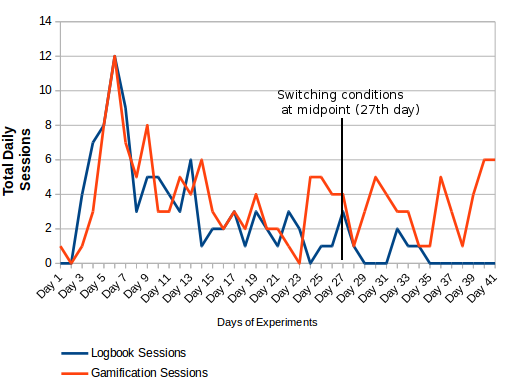
\includegraphics[width=0.6\textwidth]{Figures/scatter_daily_sessions.png}
    \rule{35em}{0.5pt}
  \caption{Comparison for trends of daily total sessions between logbook and gamification in 41 days of app usage.}
  \label{figure:usagedailysessions}
\end{figure}

\begin{table}[h!]
  \begin{center}
    \caption{Daily usage comparison between logbook and gamified systems for 41 days.}
    \label{table:usagedays}
	\begin{tabular}{|L{2.5cm}|c|c|c|c|c|c|}
		\hline
		Groups&N (days)&Mean&Sum Ranks&U&Z&P\\
		\hline
   		Daily logbook sessions&$41$&$33.72$&$1701.5$&\multirow{2}{*}{$1159.5$}&\multirow{2}{*}{$-2.9538$}& \multirow{2}{*}{$0.00318$}\\\cline{1-4} 
   		 		    Daily gamification sessions&$41$&$49.28$&$1701.5$&&&\\
\hline
	\end{tabular}
  \end{center}
\end{table}

\begin{figure}[htbp]
  \centering
    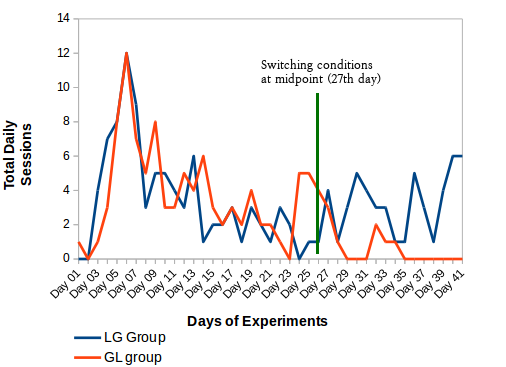
\includegraphics[width=0.6\textwidth]{Figures/usagedailysessions_lg_gl.png}
    \rule{35em}{0.5pt}
  \caption{Comparison of daily total sessions between LG group and GL group in 41 days of app usage.}
  \label{figure:usagedailysessions_lg_gl}
\end{figure}
\subsubsection{The Impact of Gamification Features on Internalization}\label{dim2}
An interesting phenomenon that expands on the usage pattern of Figure \ref{figure:usagedailysessions} is that of Figure \ref{figure:usagedailysessions_lg_gl}, which shows the usage trends of the LG (logbook-gamification) and GL (gamification-logbook) groups. It can be observed that there is a sudden drop in the number of usage sessions for users/pairs in the GL group after they switched from the gamification app to the logbook app. This pattern suggests that most behaviour regulation during the gamification condition was ego-involved (introjected) regulation. This hypothesized situation is supported by a further exploration of the number of impressions on gamification features. On checking the average impressions among the four gamification features, leaderboard had the highest average number of impressions, as shown in Figure \ref{figure:gamification_impressions_latest_all}. 
\begin{figure}[htbp]
  \centering
    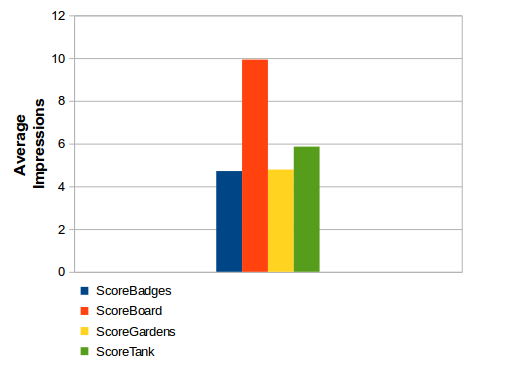
\includegraphics[width=0.6\textwidth]{Figures/gamification_impressions_latest_all.png}
    \rule{35em}{0.5pt}
  \caption{Total daily impressions for two groups (LG and GL).}
  \label{figure:gamification_impressions_latest_all}
\end{figure}
I conducted statistical comparisons on the number of impressions between leaderboard and each of the other gamification features (score badges, botanical garden and fish tank). The findings indicated that the number of impressions was significantly higher statistically for leaderboard ($Mean=9.93$, $SD=13.90$) than score badges ($Mean=4.71$, $SD = 5.50$) ($t (13) =2.1747$, $p=0.0487$). There was no statistical significance in either the number of impressions on leaderboard ($Mean=9.93$, $SD=13.90$) compared with botanical garden ($Mean = 4.79$, $SD = 5.26$) ($t(13)=1.716$, $p= 0.1096$) or the number of impressions on leaderboard ($Mean= 9.93$, $SD = 13.90$) compared with fish tank ($Mean=5.86$, $SD=7.40$) ($t(13)=1.5707$, $p = 0.1403$). However, the trend showed the dominance of leaderboard over other gamification features. 

A further exploration of gamification features' impressions revealed some insights on the trend of promotion of ego-involved and task-mastery climates. This exploration follows the discussion in the previous chapter (Chapter \ref{prototype2chapter}), where I observed that some statements from qualitative feedback reflected that gamification features tended to promote either a task-mastery climate or an ego-involved climate. In that discussion, the leaderboard tended to promote the ego-involved climate for some intermediary users, while features like the fish tank or botanical garden were inclined to promote the task-mastery climate. Literature suggests that the promotion of a task-mastery climate may foster integrated internalization of behaviour regulation, while the promotion of an ego-involved climate may only promote the introjected internalization of behaviour regulation~\citep{saksono2015spaceship}.

Since perceived usefulness is the only predictor of internalization (refer to the discussion on questionnaires in subsection \ref{methodsquestionnaire}), one of the logical steps was to compare perceived usefulness scores between intermediary users who had visited the leaderboard more often than other gamification features (i.e. the number of impressions on the leaderboard was greater than the number of impressions on any of the other gamification features) and those intermediary users whose number of impressions on the leaderboard was similar to or less than the number of impressions on any of the other gamification features. Since the average number of impressions on botanical garden, score badges and fish tank were fairly similar, as indicated in Figure \ref{figure:gamification_impressions_latest_all}, I selected only the botanical garden as a point of reference (to represent features that may promote a task-mastery climate) for comparison with leaderboard (to represent those features that may promote an ego-involved climate). 

Perceived usefulness concerned how intermediaries rated the usefulness of the app to them and their parents. I made an assumption based on literature that if the regulation was introjected, then the intermediaries would care less about the usefulness of the app. Therefore, the next task was to compare perceived usefulness between those intermediary users with high leaderboard impressions relative to the botanical garden and those with low leaderboard impressions relative to the botanical garden. In order to know whether an intermediary user fell into the high or low group, I computed a ratio by dividing the number of impressions on the leaderboard by the number of impressions on the botanical garden. After the computation of ratios, I divided 14 intermediary participants into two groups based on whether their ratio was below or above the median ($0.91$). As a result, I assigned seven intermediary users to a group with $ratio\geq Median$, while the remaining seven intermediary users were put into a group with $ratio<Median$. The next step compared perceived usefulness of the gamified app between intermediary users with $ratio \text{ of impressions }\geq Median$ and intermediary users with $ratio \text{ of  impressions }<~Median$. The two independent samples followed a normal distribution. Table \ref{table:pu_leaderboard_bias} shows the outcome  of a student-t test, which indicates that the group with $ratio<Median$ scored significantly higher in perceived usefulness than the group with $ratio\geq Median$. The implication of this finding is that those who had never accessed the leaderboard, or had accessed it fewer times relative to the botanical garden, had a higher tendency to view the intervention that utilized the gamified app as useful, compared to those who had used the leaderboard more than the botanical garden. 

\begin{table}[h!]
  \begin{center}
    \caption{Comparison of perceived usefulness between group with $ratio~\geq\textbf{Median}$ and group with ratio~\textless~\textbf{Median} (ratio = impressions on leaderboard/impressions on botanical garden).}
    \label{table:pu_leaderboard_bias}
	\begin{tabular}{|c|c|c|}
		\hline
		Mean &Group with ratio~\textgreater=~\textbf{Median}&Group with ratio~\textless~\textbf{Median}\\
		\hline
		 \multirow{2}{*}{Perceived usefulness}&$Mean=4.143$ ($SD = 0.763$)&$Mean=5.171$ ($SD = 0.962$)\\\cline{2-3} 

		 &\multicolumn{2}{|l|}{$t(12)=2.2156$, $p=0.0468$, 95\% $CI = -2.040 \text{ to }  -0.017$} \\
\hline
	\end{tabular}
  \end{center}
\end{table}

Since usage of leaderboard showed a significant decrease in scores of perceived usefulness, the next task was to see if that affected the gamification condition in general. Let's examine the trend of intermediaries' perceived usefulness between midpoint and endpoint for both the group with $ratio \geq Median$ and the group with $ratio \leq Median$. An earlier assumption was that the relationship between parents and children would make children view the app as meaningful; hence the regulation would be considered either identified or integrated regulation. But from the findings above, the trend indicated that most users concentrated on the leaderboard and, as a result, those with a higher number of impressions on the leaderboard than other gamification features such as the botanical garden had low scores in perceived usefulness.

In order to verify the significance of the aforementioned trend on impressions, I began with the hypothesis that gamification affected the perceived usefulness of the app through its leaderboard feature.  The first logical step was to assess perceived usefulness between midpoint and endpoint for the two aforementioned groups. The perceived usefulness was significantly higher at endpoint (Mean = 5.4, SD = 1.058) than midpoint ($Mean=4.67$, $SD=1.37$) ($t(6)=4.9670$, $p=0.0025$) for the group with $ratio<Median$, while for the group with $ratio>=Median$, there was no statistically significant difference between endpoint ($Mean=4.34$, $SD=1.081$) and midpoint ($Mean=4.66$, $SD=0.781$) ($t(6)=0.8742$, $p= 0.4156$). The intermediary user with the highest ratio was the one with the lowest scores on perceived usefulness. There was a negative correlation between ratio of impressions (leaderboard/botanical garden) and perceived usefulness without statistical significance ($r=0.52$, $p=0.06$, $N=14$).

What can be concluded so far from the trend on number of impressions is that it is very likely that the leaderboard played a role in hindering internalization, since perceived usefulness is a good predictor of internalization. High usage of leaderboard also suggests that most usage in gamification was, on account of ego-involved, introjected regulation.~The presence of introjected regulation is supported by the excerpt from one participant shown in Table \ref{table:introject_reg}, but it emerged in most of the excerpts of users while in the gamification condition. Therefore, usage in such cases was mostly influenced by the desire to dominate others in the competition. These different analyses support the conjecture of Figure \ref{figure:usagedailysessions} about the presence of introjected regulation due to a sudden drop in usage by pairs in the GL group  after day 27. If internalization was on the levels of identified and integrated regulations, then there would have been no sharp drop, but rather a steady one.  

\begin{table}[h!]
\renewcommand{\baselinestretch}{1.5}
  \begin{center}
    \caption{Excerpt: an example of introjected regulation.}
    \label{table:introject_reg}
	\begin{tabular}{|l|C{12cm}|}
		\hline
		No.&Comment\\
		\hline
		1.&\userquote{\textbf{Ayesha}, a beneficiary working with her son, 35 yrs} {``We [with Keagan] were not talking to others because all we wanted was to win. We didn't want them to know but they could see from the app.''}~\citep{katule2016family}\\
		\hline
	\end{tabular}
  \end{center}
\end{table} 

\subsubsection{Pairwise Comparison Between Logbook and Gamification}\label{dim3}
A different dimension of usage analysis looked at whether there was a significant difference in the number of sessions between the two experimental conditions (repeated measures of the same pairs in logbook and gamification conditions). As highlighted in the section above that describes the methods, the four pairs with technical glitches were excluded in order to make the comparison of the two experimental conditions fair (Table \ref{table:usageproblems}). The analysis showed that the means of logarithmic transformed data of normalized number of sessions between gamification and logbook were significantly different ($t(9)=2.6593$, $p=0.0261$)~\citep{katule2016family}. This implies that the number of times the app was used per day during the gamified condition was significantly higher than when pairs were in the logbook condition. The log mean had to be used in this comparison because the test for normality on differences of data points between logbook and gamification failed. A natural logarithmic transformation rectified the situation.

The next sub section report on user experiences of both intermediaries and beneficiaries.
\subsection{Intermediaries' User Experience}\label{interm_user_xp}
In most cases, the intermediary user facilitated usage of the app through proximate enabling and proximate translation. The work of~\cite{sambasivan2010} discussed these types of intermediated interactions. Baseline data indicated that intermediary participants had more interest in using cellphones than beneficiary participants. For instance, in an overall IMI scores to use a cellphone, intermediaries ($Mean=5.76$, $SD=0.41$, $N=14$) scored  significantly higher than beneficiary participants ($Mean=5.06$, $SD= 0.71$, $N=13$) with ($t(25)=3.1764$, $p=0.0039$).

If one refers back to the trend in Figure \ref{figure:usagedailysessions_lg_gl}, during the initial days of the experiment both gamification and logbook had patterns that were similar. However, after the second week, logbook usage started to go down while the trend for gamification remained steady for a couple of days. One of the possible explanations for why logbook had the same trend as gamification at the beginning is because both experimental conditions experienced the novelty effect which wore off after a few days. Also, the effect of having access to a smartphone contributed to high usage to most of the intermediary users in the logbook condition during phase 1 of the experiment. The act of sharing a phone during the intervention was important for nurturing the relationship between intermediaries and beneficiaries. In cases where parents shared the intervention's phone with their children, the children tended to be more interested in the intervention. Free access to the intervention's phone played a role in increasing the engagement of intermediary participants who did not have their own smartphones or data bundles in their smart-phones. In some cases, intermediary users installed and utilized other apps on the intervention's phones, such as games and social networks. To understand how the phone had a strong effect on motivation, I explored the relationship between perceived autonomy to use the cellphone at baseline and perceived enjoyment of using the Family Wellness app at midline for the group that started with the logbook. This exercise revealed an interesting phenomenon: there was a significant negative relationship between perceived autonomy to use a cellphone at baseline and perceived enjoyment of using the app at midline for the LG group ($r=-0.84$, $p=0.017$, $N=7$). A possible explanation for this is that those intermediary users with low autonomy to use a cellphone suddenly had free access to the intervention phone, and this increased their interest to participate in the intervention. For instance, one intermediary user (\textbf{Siphosethu}) from the LG group, who was the youngest participant (12 years of age), reported the lowest score in perceived autonomy to use a cellphone at baseline, and the highest score in  perceived enjoyment of using the app at midpoint (after using the logbook condition). She reported that she had freedom to use the intervention's phone as shown by the excerpt in Table \ref{table:interm_freed}.

\begin{table}[h!]
\renewcommand{\baselinestretch}{1.5}
  \begin{center}
    \caption{Excerpt: an example of a participant with freedom to use the intervention's phone.}
    \label{table:interm_freed}
	\begin{tabular}{|l|C{12cm}|}
		\hline
		No.&Comment\\
		\hline
		1.&\userquote{\textbf{Siyamthanda}, an intermediary} {``I had freedom because sometimes she left the phone with me and I was able to play games''}~\citep{katule2016family}\\
		\hline
	\end{tabular}
  \end{center}
\end{table}

There was an indication that having access to a phone, coupled with the novelty effect, had mediated engagement of some intermediaries that had started with the logbook condition. These intermediaries were helping their parents, and in return they had a free pass to access the intervention's cellphone. This finding is inconclusive due to the limited sample size; however, it highlights what could be explored in future studies. For the GL group it was difficult to isolate the gamification effect from the phone and novelty effect -- literature suggests that gamification has a novelty effect too~\citep{koivisto2014demographic}, for example. However, the trend shows that gamification accumulated more sessions compared to logbook, hence gamification alone increased utilization of the Family Wellness app. Gamification appeared to be the most dominant factor, that influenced usage, as we have already seen that the frequency of usage was higher in gamification than in logbook.

In addition to the novelty and phone effects, and gamification, another factor that contributed to intermediaries' interaction with the Family Wellness app was requests from beneficiaries. There were times when intermediary users opened the app for interaction only upon receiving requests from beneficiaries. In both absence and presence of gamification, intermediaries had to fulfil requests from beneficiaries.  But during the logbook condition, intermediaries appeared to be less enthusiastic in handling those requests. Some beneficiaries complained that there were several instances when their intermediary users refused to fulfil these requests, and this happened more often during the logbook condition. I had observed that in most of these cases, intermediary participants' autonomy was violated as requests came at times when intermediary participants were either studying for exams or doing something else, and they felt it was not the right time to fulfil those requests. As a result, some intermediary participants felt nagged by their parents. This happened during the logbook condition or in cases where gamification was demotivating for intermediary users who had not made progress~\citep{katule2016family}.

I categorized motivational drivers for all the requests that were put forward by beneficiary users to be originating from two main sources The first source of motivation was the instrumental value derived from using the app. The second source was gamification. Requests that were mediated by gamification fostered a sense of collaboration between members of a pair, while in the scenarios where beneficiaries were not concerned about gamification, or during the logbook condition, requests tended to be of an authoritative nature~\citep{katule2016family}. %Therefore the presence of gamification in this context tended to promote a collective responsibility for pairs where both members of a pair were motivated by gamification unlike in logbook condition where there was an absence of that cooperation.

\begin{table}[h!]
\renewcommand{\baselinestretch}{1.5}
  \begin{center}
    \caption{Excerpt: how gamification promoted collaboration.}
    \label{table:promote_collabo}
	\begin{tabular}{|l|C{12cm}|}
		\hline
		No.&Comment\\
		\hline
		1.&\userquote{\textbf{Ayesha}, a beneficiary}{``I would always ask him [Keagan] `Where are we. Are we first? And what badge do we have? Where are the others? How far is Simon [intermediary] then? How far is that one?' `No Mum, we are on top. We are first. We are the champions' [during gamification].''}~\citep{katule2016family} \\
		\hline
	\end{tabular}
  \end{center}
\end{table}

The excerpt from \textbf{Ayesha} (Table \ref{table:promote_collabo}) demonstrates a sense of collaboration between the two members of a participating pair (\emph{Ayesha} and \emph{Keagan}). The presence of gamification in this context tended to promote a collective responsibility for pairs (a sense of collectivism), where both members of a pair were motivated by gamification, unlike in the logbook condition where there was an absence of that cooperation. The excerpt shown in Table \ref{table:authoritarian} came from a beneficiary participant in the logbook condition and it indicated that she initiated usage while showing a sense of authority; it was not a cooperation between members of the pair. 

\begin{table}[h!]
\renewcommand{\baselinestretch}{1.5}
  \begin{center}
    \caption{Excerpt: a beneficiary demonstrating a tendency of being authoritative.}
    \label{table:authoritarian}
	\begin{tabular}{|l|C{12cm}|}
		\hline
		No.&Comment\\
		\hline
		1.&\userquote{\textbf{Sisipho}, a beneficiary working with her son, 43 yrs} {``I always start the conversation. Because I always want to make sure if he records because I can't use it. It was difficult for me to use it [during logbook].''}~\citep{katule2016family}\\
		\hline
	\end{tabular}
  \end{center}
\end{table}

The gamified app was designed in such a way that a pair would earn rewards based on cooperation between members: usage controlled by the intermediary participant and the average number of steps walked by the beneficiary participant (see more details in section \ref{prototype2descr}). The purpose of rewards was to foster users' intrinsic experiences such as competitiveness and a sense of autonomy, which are main contributors for intrinsic motivation, with the goal of improving collaboration between members of a pair. The presence of gamification nurtured teamwork even though the regulation of self-monitoring through intermediary users was mostly introjected (regulation done for the purpose of becoming better than others), as shown by the excerpts in Table \ref{table:introject_regulation2}.

\begin{table}[h!]
\renewcommand{\baselinestretch}{1.5}
  \begin{center}
    \caption{Excerpts: examples of teamwork as a result of competition from others.}
    \label{table:introject_regulation2}
	\begin{tabular}{|l|C{12cm}|}
		\hline
		No.&Comment\\
		\hline
		1.&\userquote{\textbf{Keagan}, an intermediary for his mother, 16 yrs} {``When I see other people trying to come above me [on the leaderboard], I hand over the phone to my mom so she can walk more steps.''}~\citep{katule2016family}\\
		\hline
		2.&\userquote{\textbf{Christine}, an intermediary for her mother, 16 yrs} {``I told my mom that me myself I want our team to have the highest points. `Yes', she said, she is going to do that.''}~\citep{katule2016family}\\
		\hline
	\end{tabular}
  \end{center}
\end{table}

Through these collaborations, goals were set. In most cases they were set by the intermediary user, who informed their beneficiary about what they wanted the team to do (excerpts in Table \ref{table:goal_formulation}); a pattern shown in Chapters \ref{prototype1chapter} and \ref{prototype2chapter} repeats itself for these intermediaries: a sense of joint ownership of the whole process in using the app. 

\begin{table}[h!]
\renewcommand{\baselinestretch}{1.5}
  \begin{center}
    \caption{Excerpts: examples of intermediaries suggesting goals for their team.}
    \label{table:goal_formulation}
	\begin{tabular}{|l|C{12cm}|}
		\hline
		No.&Comment\\
		\hline
		1.&\userquote{\textbf{Sophia}, an intermediary for her mother, 17 yrs} {``Sometimes that person may be first so I tell my mom that we must also be at the first place. [She looks at the  leaderboard and sees other people in the first place, and tells her mother that they should also aim for first position].''}\\
		\hline
		2.&\userquote{\textbf{Jenner}, a beneficiary working with her son, 45 yrs} {``When he [15-year-old Leon] looked through it [The app] and saw their points, he would say `Mom, we need to do something here, because look at their points and our points'. So it was quite interesting.''}\\
		\hline
	\end{tabular}
  \end{center}
\end{table}

Comparison of virtual rewards among intermediary users motivated them to check the app more often, compared with when they were in the logbook condition, as highlighted in the usage findings (subsection \ref{usageoutcome}). Intermediaries competed which each other through the leaderboard, and as a result there were frequent face-to-face interactions that entailed comparing scores, since most of the intermediary participants who lived in the same study's site (Langa or Athlone), either attended the same schools or lived not far from each other. The presence of these face-to-face interactions is shown an the excerpt in Table \ref{table:interm_facetoface}. These face-to-face interactions have been common throughout all evaluations reported in the previous chapters, as result in some situations, either the social features implemented in the app were never utilized or they were infrequent utilized. This part is revisited when presenting findings on relatedness, and it is further expanded in the discussion section, on its implications to the design of systems that encourage social comparison. 

\begin{table}[h!]
\renewcommand{\baselinestretch}{1.5}
  \begin{center}
    \caption{Excerpt: an example of face-to-face interactions between intermediaries.}
    \label{table:interm_facetoface}
	\begin{tabular}{|l|C{12cm}|}
		\hline
		No.&Comment\\
		\hline
		1.&\userquote{\textbf{Jenner}, a beneficiary} {``He [Leon] likes this exercise [using the app] because among him and his friends, they would have that competition like `I got more points than you' and that motivated him to get interested with the app.''}\\
		\hline
	\end{tabular}
  \end{center}
\end{table}
 
In most of the cases presented above, the pattern suggests that regulation was mostly introjected, as it was mediated by the need to be better than other participants in terms of points or being at the top of the leaderboard. This comparison among participants obscured the presence of other features to a great extent; this is proved by the fact that these features were not discussed in detail in the interviews, as intermediary users or beneficiary users who the researcher interviewed did not give any insights. The desire to be better than other participants led to cheating in some cases. For instance, in one pair, the beneficiary user and the intermediary user took turns to use the pedometer, therefore accumulating more steps and more points (Table \ref{table:cheating}). 

\begin{table}[h!]
\renewcommand{\baselinestretch}{1.5}
  \begin{center}
    \caption{Excerpt: an example of a case where steps were accumulated by both members of a pair.}
    \label{table:cheating}
	\begin{tabular}{|l|C{12cm}|}
		\hline
		No.&Comment\\
		\hline
		1.&\userquote{\textbf{Christine}, an intermediary for her mother, 16 yrs} {``I ask her `How far did you walk?' She would say she walked very far. She tells me that I must have the phone to walk more steps. She would say `I got more walking than you' [mother and daughter were collaborating in accumulating steps]. She sometimes writes the steps on the page and she tells me `Yesterday I had more points than you [points referring to steps]'.''} \\
		\hline
	\end{tabular}
  \end{center}
\end{table} 

Competition appeared to also affect pairs that had started with the logbook condition. Some intermediary users pushed their beneficiaries to do more, expecting rewards once they switched to the gamification condition. As a result, during the logbook condition there were intermediary participants who showed ambition to win while conversing with their respective beneficiaries~\citep{katule2016family}. The presence of gamification was also inclined to strengthen the family bond or relatedness between members of a participating pair (Table \ref{table:related_increase}).

\begin{table}[h!]
\renewcommand{\baselinestretch}{1.5}
  \begin{center}
    \caption{Excerpt: an example of an increase relatedness between members of a pair.}
    \label{table:related_increase}
	\begin{tabular}{|l|C{12cm}|}
		\hline
		No.&Comment\\
		\hline
		1.&\userquote{\textbf{Khanyiswa}, a beneficiary working with her daughter, 26 yrs} {``I think we talk more [with \textbf{Siphosethu}] than before the Family Wellness app. Before the Family Wellness app, after work it was just `Hi' and then I go to my room. But now she would come to my room  and say `Let me see your phone. What did you eat today?' and write everything down on the phone.''}\\
		\hline
	\end{tabular}
  \end{center}
\end{table} 

When it came to relatedness among intermediary users, social features were infrequent utilized: only two users showed interests towards such features. One of those two users appeared to attempt to make a social connection with other users through the app. It was observed that this particular user was not in physical contact with other users, hence using social features on the app was the only way to feel connected with others. One of the comments made by this user, to a fish tank that belonged to the other team is as shown in Table \ref{table:social_features}.

\begin{table}[h!]
\renewcommand{\baselinestretch}{1.5}
  \begin{center}
    \caption{Excerpt: an example of utilization for social features in the app.}
    \label{table:social_features}
	\begin{tabular}{|l|C{12cm}|}
		\hline
		No.&Comment\\
		\hline
		1.&\userquote{\textbf{Siphosethu}, an intermediary} {``Wow it shows that you are working hard  Clara\#2. [congratulating [Clara a female intermediary aged 14 years, for having her fish tank ranked number 2 in quality.]''}\\
		\hline
	\end{tabular}
  \end{center}
\end{table}    

The overall findings on user experience indicated mixed results, with some intermediary users having a positive experience while utilizing gamification, while the perceived enjoyment of some intermediary users was lower in gamification compared with logbook, despite the fact that there were more sessions reported in gamification. A leaderboard can indeed demotivate users at the bottom, but it can also foster aspects of relatedness for all users~\citep{sailer2013:psychological}. Since the leaderboard drew most attention, it could have played a role in demotivating users with lower performance. Therefore, in looking for evidence that supports this conjecture, I analysed the trend for both perceived enjoyment and usage, for each of the 14 intermediaries. As a result, I was able to identify several intermediary users whose trend for user experience showed a pattern worth discussing here. The process is as explained in the next paragraphs.

If we refer to the way the experiments were set, there were seven intermediaries in gamification, for each of the two phases of the experiment (phase 1: weeks 1\thinspace-\thinspace4, and phase 2: weeks 5 and 6). As a result, at any point of time, the leaderboard had seven teams. I went ahead to defining the criterion for identifying teams that were considered at the bottom, as the word bottom was vague. I looked for the teams that achieved only one badge (the lowest of all available badges) throughout the gamification condition; five teams in total were identified from both phases. Table \ref{table:bottom} shows the resulting list of teams at the bottom. The order of this list cannot be interpreted as pair's respective position on the leaderboard. Let's just view these teams as the bottom ones according to their respective leaderboard in either phase 1 or phase 2. The list also shows the total number of days that each team utilized the leaderboard and the change in the intermediaries' perceived enjoyment scores between gamification and logbook. A negative change means the score in gamification was lower than logbook, while a positive change means the score in gamification was higher than logbook. A negative change implies that, gamification harmed intrinsic motivation -- perceived enjoyment is the direct measure for intrinsic motivation. 

\begin{table}[h!]
  \begin{center}
    \caption{Pairs at the bottom of the leaderboard.}
    \label{table:bottom}
	\begin{tabular}{|c|c|c|c|c|c|}
		\hline
		&\multirow{2}{*}{Pair}&Intermediary's  & Group &Leaderboard's& Change in perceived\\
         &&pseudonym&sequence&visits (days) &enjoyment scores\\	
		\hline
		1&Pair-C&Lelethu&LG&0&1\\
		\hline
		2&Pair-D&Lindela&LG&2&-1.58\\
		\hline
		3&Pair-E&Leon&GL&4&-2.42\\
		\hline
		4&Pair-F&Keller&LG&4&-0.42\\
	\hline
		5&Pair-G&Jaquan&LG&1&0.25\\
	\hline
	\end{tabular}
  \end{center}
\end{table}

The findings in Table \ref{table:bottom} above, suggests that the negative change in motivation is observed in three intermediary users that accessed the leaderboard for at least two days. The simple explanation for the trend is that, users spent their first day of usage in trying to familiarise themselves with the gamification features. For those who came back to the leaderboard after the first day, it was because of the interest in comparing performance between them and others. Two users showed positive change: Lelethu (a 16-year-old male) and Jaquan (an 18-year-old female), but did not fully engage with the leaderboard (zero days for Lelethu and one day for Jaquan) like their peers at the bottom's list. Let's now answer the question for how the remaining three intermediaries, namely Keller (a 13-year-old male), Lindela (a 17-year-old male) and Leon, were negatively affected by the leaderboard. Let's start by reviewing Lindela's case first. Lindela's pair had their pedometer malfunctioned. The same situation happened to Lelethu, but unlike Lindela, his score on perceived enjoyment was higher in gamification than logbook. The two users had also shown more efforts in interacting with the logbook app before they switched to gamification; this is supported by a testimony from a 16-year old Anathi, who explained how unsure she was of the credibility of the gamified system, because her peers appeared to have more interest in the app but were at lower positions on the leaderboard than her (Table \ref{table:credibility}).

\begin{table}[h!]
\renewcommand{\baselinestretch}{1.5}
  \begin{center}
    \caption{Excerpt: an example of how technical glitches reduced the credibility of the app.}
    \label{table:credibility}
	\begin{tabular}{|l|C{12cm}|}
		\hline
		No.&Comment\\
		\hline
		1.&\userquote{\textbf{Anathi}, an intermediary for her mother} {``It [the experience of using the gamified app] was the same as last time [during the logbook condition] except for the game part. I was actually above some of the others. That was weird. Because they were more interested in the app than me. [She was making a reference to the two intermediary users that were found to be experiencing problems with their pedometers: Lindela and Lelethu. The three lived nearby each other''} \\
		\hline
	\end{tabular}
  \end{center}
\end{table}     

Anathi expected her peers to be more competent than her once she switched to gamification. Contrary to her expectations she was ahead of them, and this made her doubt her competence. This is further shown by her reported score on perceived competence in logbook and in gamification, where she reported lower score in gamification compared to logbook, despite using gamification for seven out of 14 days and logbook for only four out of 27 days. However, Anathi reported a slightly higher perceived enjoyment score  during gamification than logbook. This excerpt by Anathi together with the usage logs, suggest that an intermediary user from Pair-C (Lindela) was negatively affected with the leaderboard as a result of technical glitches. For Lelethu, his absence of contact with the leaderboard improved her perceived enjoyment in using the app while in the gamification condition. Also in this case, it is also clear that, technical glitches not only negatively affected the motivation of some intermediary users, but it also raised questions about credibility of the app. System credibility support has been highlighted as one the four important aspects of persuasive system design~\citep{Oinas-kukkonen:psd}. 

\begin{figure}[htbp]
  \centering
    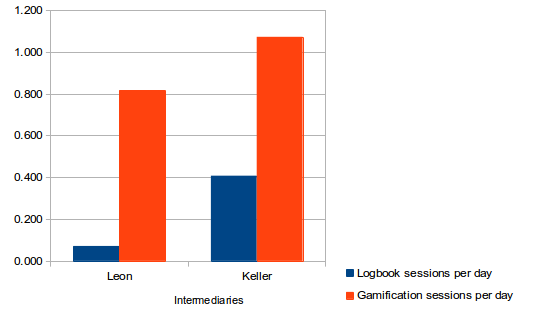
\includegraphics[width=0.5\textwidth]{Figures/badgesfailures2.png}
    \rule{35em}{0.5pt}
  \caption{Usage of two pairs with lack of progress in badges due to insufficient number of footsteps.}
  \label{figure:badge_failure_2}
\end{figure} 

The leaderboard also affected intermediary users in Pair-E and Pair-F (Leon and Keller), as a result of the app not being able to tailor challenges to the skills of the intermediary users. Their beneficiary participants were not walking enough steps, despite the fact that these two intermediaries had put more efforts into using the app during the gamification condition than in the logbook condition as shown in Figure \ref{figure:badge_failure_2} above; this means the two users were more eager to engage with the app in the gamification condition than logbook, but were let down by their beneficiaries. Their performance relied to a great extent on the performance of their respective beneficiary users. For the intermediary users in this case , their negative experience was assumed to be the result of the gamification design's failure to match challenges with abilities. The efforts of their beneficiary differed from their own, and this had an effect on the overall performance of the team. In that context, intermediary users had little control over the performance of their beneficiaries. Some intermediaries reacted negatively when they thought their beneficiary was not complying with carrying the pedometer when they should (Table \ref{table:negativereact}). 

\begin{table}[h!]
\renewcommand{\baselinestretch}{1.5}
  \begin{center}
    \caption{Excerpt: an example of negative reaction that threatened the social relationship between members of a pair.}
    \label{table:negativereact}
	\begin{tabular}{|l|C{12cm}|}
		\hline
		No.&Comment\\
		\hline
		1.&\userquote{\textbf{Jenner}, a beneficiary} {``Sometimes maybe I forget to take the phone when I go walking and he [Leon] would ask me `Did you take the phone with you?' `Ooh Gosh I forgot.'  Because when I walk to Park Town to exercise, sometimes  I am in such a hurry I forget the phone, and he gets crossed with me.''}\\
		\hline
	\end{tabular}
  \end{center}
\end{table} 

The excerpt above, demonstrates how an intermediary user was attempting to control his beneficiary user as a result of competition with intermediary users in other pairs. Instead of gamification being something enjoyable in this context it had a negative result that threatened the existing social rapport between parent and child. The exposure to the leaderboard contributed to the frustrating situation of not progressing. At one point, Leon contacted the researcher, because he wanted to know what else he needed to do in order to progress in the game. This suggests that challenges and skills were far apart.

In comparing the support of the three basic psychological needs in logbook and gamification, I made a decision to exclude four intermediary users, whose perceived enjoyment was largely affected by either technical glitches or exposure to the leaderboard coupled with the inability to participate fairly in gamification because of either the pedometer not working or design limitations of the app. The first three intermediaries have already been discussed above: Lindela (Pair-D), Pair-E (Leon) and Keller (Pair-F). The fourth intermediary user on the list is from Pair-A in Table \ref{table:usageproblems}. The technical glitches negatively affected his whole user experience of using the app and this happened during the gamification condition. His experience is reflected by the message in Table \ref{table:negativexp} that he sent to the researcher. The message was sent on the 11\SP{th} day since the beginning of the experiment, through the chat room that was available on the app. 

\begin{table}[h!]
\renewcommand{\baselinestretch}{1.5}
  \begin{center}
    \caption{Excerpt: an example of negative user experience due to technical glitches.}
    \label{table:negativexp}
	\begin{tabular}{|l|C{12cm}|}
		\hline
		No.&Comment\\
		\hline
		1.&\userquote{\textbf{Nathan}, an intermediary for his father, 20 yrs} {``Chief! [Chief -- a nickname for the researcher] This app is unstable. Kicks me out for days, stops running, doesn't respond, exits when orientation changes and the list goes on. As for the pedometer, that too has bugs. It crashes or sometimes freezes (doesn't respond), makes it difficult to use the app.''}\\
		\hline
	\end{tabular}
  \end{center}
\end{table}    

The decision to exclude the four pairs above, aimed to minimize the negative effect of extraneous factors in reducing the power of the study, in detecting differences in motivation scores between the logbook condition and the gamification condition. These extraneous factors were: weak design  for gamification -- as the system lacked the ability in supporting adaption of challenges to skills, and the unexpected technical problems that affected the overall user experience. 

As a result of excluding the scores of four intermediary participants, only 10 out of 14 intermediary users were considered in the subscales that measured the three aspects of SDT (autonomy, competence and relatedness). On perceived competence in using the app, the gamified condition scored significantly higher than the logbook condition ($t(9)=3.495$, $p=0.0068$)~\citep{katule2016family}. There was no significant difference between logbook and gamification scores of perceived autonomy ($t(9)=0.027$, $p=0.98$) and perceived relatedness ($t(9)=0.719$, $p=0.49$)~\citep{katule2016family}.

\subsection{Beneficiaries' User Experience}\label{ben_user_xp}
As most beneficiaries only interfaced with the app through intermediary users, beneficiaries' user experience relied on cooperation from intermediaries. Concerning support for the three basic psychological needs, there was no difference between logbook and gamification. However, relatedness ($N=14$) appeared to improve significantly with time between midpoint ($Mean=4.43$, $SD=0.92$) and endpoint ($Mean=5.38$, $SD=1.08$)($t(13)=2.3736$, $p=0.0337$). Therefore, the intervention in general made beneficiaries feel more related to others (their respective intermediaries and other beneficiaries) who were part of the intervention.
  
When utilizing the app through intermediaries, there were cases where beneficiaries had a negative experience as a result of intermediaries refusing to assist when asked to. This happened in cases where intermediary users did not feel like helping, either because they were occupied by other tasks such as learning for exams, or because they felt the app was boring, especially in the logbook condition. 

In the next subsection, the IMIs in the self-monitoring of diet and activity are reported on. Four pairs with usage problems (Table \ref{table:usageproblems}) were excluded due to their self-monitoring being affected. Therefore, in total only 10 out of 14 beneficiaries had their results included for analysis, in order to have only beneficiaries who had meaningful engagement with the app through their respective intermediaries.
\subsubsection{IMI in Self-Monitoring of Diet}
The results for self-monitoring of diet (baseline, midline and endline) are shown in Table  \ref{table:imidietbenf}. The Mauchly’s test indicated that the assumption of sphericity was not violated with  $\chi{}^2(2)=3.76$, $p=0.152$. The results ($N=10$) on self-monitoring of diet shown in Table \ref{table:imidietbenf}, were from sphericity assumed output. ANOVA showed that there was a significant difference in average IMI scores for self-monitoring of diet measured at baseline, midline and endline.
\begin{table}[h!]
  \begin{center}
    \caption{Comparison of 10 beneficiaries' IMI scores in self-monitoring of diet at baseline, midline and endline.}
    \label{table:imidietbenf}
	\begin{tabular}{|L{2.8cm}|L{3.2cm}|L{3.2cm}|L{3.2cm}|}
		\hline
		Mean IMI Score &Baseline&Midline&Endline\\
		\hline
		 %\multirow{3}{*}
		 {Self-monitoring}&$Mean=4.48$, $SD=1.24$&$Mean=5.07$, $SD=1.19$&$Mean=5.55$, $S.D=0.95$\\\cline{2-4} 

		of Diet &\multicolumn{3}{|l|}{$F(2,18)=3.787$, $p=0.042$} \\
\hline	\end{tabular}
  \end{center}
\end{table}
A finding from pairwise comparisons (a paired student t-test) indicated that the IMI score at endline was significantly higher than at baseline (Table \ref{table:imipairwisediet}). The difference between baseline, midline and endline was not significant (Tables \ref{table:imipairwisediet1}, and \ref{table:imipairwisediet2}). Motivation to self-monitor diet appeared to increase with time, as shown in Figure \ref{figure:imi_diet}. The interpretation of the above findings is that the wellness app appears to have had a significant effect over time on the motivation of beneficiaries to self-monitor their diet.
\begin{table}[h!]
  \begin{center}
    \caption{Pairwise comparisons of IMI scores for self-monitoring of diet: baseline versus midline.}
    \label{table:imipairwisediet}
	\begin{tabular}{|L{2cm}|L{4cm}|L{4cm}|}
		\hline
		Mean &Baseline&Midline\\
		\hline
		 \multirow{2}{*}{IMI Score}&$Mean=4.48$, $SD=1.24$&$Mean=5.07$, $SD=1.19$\\\cline{2-3} 

		 &\multicolumn{2}{|l|}{$t(9)=1.298$, $p=0.227$} \\
\hline
	\end{tabular}
  \end{center}
\end{table}
\begin{table}[h!]
  \begin{center}
    \caption{Pairwise comparisons of IMI scores for self-monitoring of diet: baseline versus endline.}
    \label{table:imipairwisediet1}
	\begin{tabular}{|L{2cm}|L{4cm}|L{4cm}|}
		\hline
		Mean &Baseline&Endline\\
		\hline
		 \multirow{2}{*}{IMI Score}&$Mean = 4.48$, $SD = 1.24$&$Mean = 5.55$, $SD = 0.95$\\\cline{2-3} 

		 &\multicolumn{2}{|l|}{$t(9)=2.457$, $p=0.036$} \\
\hline
	\end{tabular}
  \end{center}
\end{table}
\begin{table}[h!]
  \begin{center}
    \caption{Pairwise comparisons of IMI scores for self-monitoring of diet: midline versus endline.}
    \label{table:imipairwisediet2}
	\begin{tabular}{|L{2cm}|L{4cm}|L{4cm}|}
		\hline
		Mean &Midline&Endline\\
		\hline
		 \multirow{2}{*}{IMI Score}&$Mean=5.07$, $SD=1.19$&$Mean=5.55$, $SD=0.95$\\\cline{2-3} 

		 &\multicolumn{2}{|l|}{$t(9)=1.975$, $p=0.08$} \\
\hline
	\end{tabular}
  \end{center}
\end{table}

\begin{figure}[htbp]
  \centering
    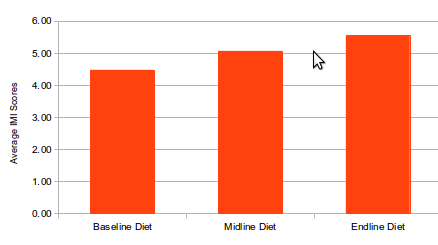
\includegraphics[width=0.4\textwidth]{Figures/imi_diet.png}
    \rule{35em}{0.5pt}
  \caption{Trend for average IMI scores for self-monitoring of diet at three points: baseline, midline and endline.}
  \label{figure:imi_diet}
\end{figure}
This ANOVA finding does not discern between the different experimental conditions which pairs of users were exposed to. The ANOVA finding (N=10) (Table  \ref{table:imidietbenf2}) on the comparison of IMI scores for the self-monitoring of diet during baseline, logbook, and gamification conditions showed that there was no significant difference in average IMI scores. This finding was a result of sphericity-assumed output of the ANOVA test, since the Mauchly’s test indicated that the assumption of sphericity was not violated with  $\chi{}^2(2)=2.19$, $p=0.335$. The trend for averages shows both logbook and gamification to be slightly higher than baseline, as shown in Figure \ref{figure:imi_diet2}. The conclusion from this finding is that both versions of the prototype cause an increase in motivation of beneficiaries to self-monitor their diet.
\begin{table}[h!]
  \begin{center}
    \caption{Comparison of 10 beneficiaries' IMI scores for self-monitoring of diet at baseline, after logbook, and  after gamification conditions.}
    \label{table:imidietbenf2}
	\begin{tabular}{|L{2.8cm}|L{2.5cm}|L{2.5cm}|L{2.5cm}|}
		\hline
		Mean IMI Score &Baseline&Logbook&Gamification\\
		\hline
		 %\multirow{3}{*}
		 Self-monitoring&$Mean=4.48$, $SD=1.241$&$Mean=5.28$, $SD = 1.05$&$Mean=5.34$, $SD=1.16$\\\cline{2-4} 
		 of Diet&\multicolumn{3}{|l|}{$F(2,18)=3.787$, $p=0.087$} \\
\hline	\end{tabular}
  \end{center}
\end{table}
\begin{figure}[htbp]
  \centering
    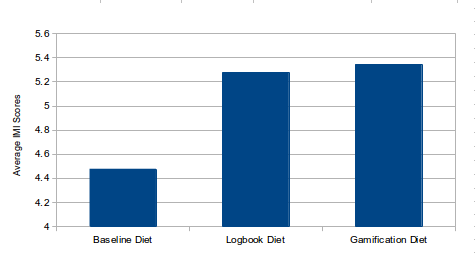
\includegraphics[width=0.4\textwidth]{Figures/imi_diet2.png}
    \rule{35em}{0.5pt}
  \caption{Trend for average IMI scores for self-monitoring of diet at three points: baseline, logbook and gamification.}
  \label{figure:imi_diet2}
\end{figure}
\subsubsection{IMI in Self-Monitoring of Activity}
The results for self-monitoring of activity are shown in Table  \ref{table:imiactivitybenf}. The results are based on a sample of nine beneficiary users, as one participant did not complete this part of the questionnaire at baseline.  The Mauchly’s test indicated that the assumption of sphericity was violated with  $\chi{}^2(2)=8.248$, $p=0.016$. The value $\epsilon$ on Greenhouse-Geisser was $<0.75$, therefore, I selected the results for self-monitoring of activity shown in Table \ref{table:imiactivitybenf} from Greenhouse-Geisser output. ANOVA showed that there was no significant difference in the average IMI scores for self-monitoring of activity measured at baseline, midline and endline. The trend of means increases from baseline to endline, as shown in Figure \ref{figure:imi_activity}.

There are several factors that might have contributed to results not being significant among baseline, midline and endline points. The first hypothesized reason is that tracking of physical activity appeared to be easy for the majority of the participants, even without tracking devices, as people can estimate the distance they walk daily and they consider this to be tracking, even though they might not have means to record this information. Hence participants' motivation was high at baseline, unlike diet self-monitoring, which they considered to be cumbersome due to external barriers such as healthy food being expensive and lacking of knowledge about healthy food; therefore at baseline, participants felt more motivated to track their activity. The second hypothesized reason is that the sample size was small, hence it was more difficult to detect a significant difference. But we have seen that the trend in motivation increases with time.
\begin{table}[h!]
  \begin{center}
    \caption{Comparison of 10 beneficiaries' IMI scores for self-monitoring of activity at baseline, midline and endline.}
    \label{table:imiactivitybenf}
	\begin{tabular}{|L{2.8cm}|L{2.5cm}|L{2.5cm}|L{2.5cm}|}
		\hline
		Mean IMI Score &Baseline&Midline&Endline\\
		\hline
		 %\multirow{3}{*}
		 Self-monitoring&$Mean=4.82$, $SD=1.002$&$Mean=5.28$, $SD=1.003$&$Mean=5.41$,$SD=0.894$\\\cline{2-4} 
		 of activity&\multicolumn{3}{|l|}{$F(1.182, 9.455)=2.936$, $p = 0.116$} \\
\hline	\end{tabular}
  \end{center}
\end{table}

\begin{figure}[htbp]
  \centering
    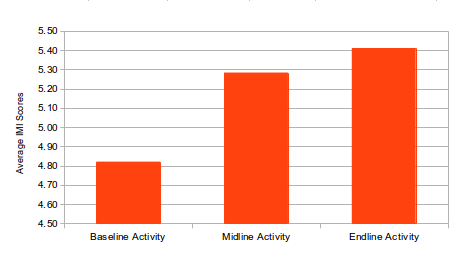
\includegraphics[width=0.4\textwidth]{Figures/imi_activity.png}
    \rule{35em}{0.5pt}
  \caption{Trend for average IMI scores for self-monitoring of activity at three points: baseline, logbook and gamification.}
  \label{figure:imi_activity}
\end{figure}
The finding from an analysis ($N=9$) where I examined if there was a difference between baseline, logbook and gamification in self-monitoring of activity, showed that there was no significant difference of average IMI scores (Table \ref{table:imiactivity2benf}). The Mauchly’s test indicated that the assumption of sphericity was violated with  $\chi{}^2(2)=6.788$, $p=0.034$. The value of $\epsilon$ on Greenhouse-Geisser was \textless 0.75; therefore, I selected the results for  self-monitoring of activity from Greenhouse-Geisser output of one-way ANOVA (with repeated measures) test. The trend in motivation increases in both logbook and gamification compared to baseline, as shown in Figure \ref{figure:imi_activity2}
%epsilon=0.617
\begin{table}[h!]
  \begin{center}
    \caption{Comparison of 10 beneficiaries' IMI scores for self-monitoring of activity at baseline, logbook and gamification.}
    \label{table:imiactivity2benf}
	\begin{tabular}{|L{2.8cm}|L{2.5cm}|L{2.5cm}|L{2.5cm}|}
		\hline
		Mean IMI Score &Baseline&Logbook&Gamification\\
		\hline
		 %\multirow{3}{*}
		 Self-monitoring&$Mean=4.82$, $SD=1.002$&$Mean=5.33$, $SD=0.9762$&$Mean=5.37$,$SD=0.9276$\\\cline{2-4} 
		 of activity&\multicolumn{3}{|l|}{$F(1.234, 9.872)=2.783$, $p=0.123$} \\
\hline	\end{tabular}
  \end{center}
\end{table}
\begin{figure}[htbp]
  \centering
    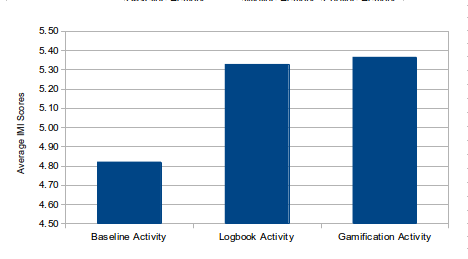
\includegraphics[width=0.4\textwidth]{Figures/imi_activity2.png}
    \rule{35em}{0.5pt}
  \caption{Trend for average IMI scores for self-monitoring of activity at three points: baseline, logbook and gamification.}
  \label{figure:imi_activity2}
\end{figure}

\section{Discussion}
\subsection{Motivational Affordances' Impact on Intermediaries}
As reported above, intermediary users facilitated interaction with the app. Intermediaries were motivated to engage with the app mostly because of two main reasons: either to follow up on competition with others, or in response to requests from their respective beneficiary users. Gamification was the main source of motivation for intermediaries. It played a pivotal role in mediating usage during the gamification condition, and even in the logbook condition for intermediary users in pairs that had started with the logbook condition before being switched to gamification. Some users who started with the logbook condition were eager to experience gamification, and this motivated them to sustain engagement while in logbook. This was true in the case of \textbf{Siphosethu}, an intermediary user who talked of winning while still in logbook condition. This affected the separation of experimental conditions, since the randomization of experimental sequences was not blind. Those that started with logbook already knew that they would start using gamification after a period of three weeks, and this positively affected their engagement with the app. On perceived competence, the difference between logbook and gamification was statistically significant, showing intermediary users in gamification felt more competent. A statistically significance difference was not seen for autonomy and relatedness, possibly due to uncontrolled interaction between experimental conditions and some other contextual factors that I have hypothesized later on this section. Perceived competence and perceived autonomy are the most important predictors of intrinsic motivation. 

From the findings it is also evident that gamification played a role in improving intermediaries' perceived enjoyment (a direct measure of intrinsic motivation) in using the app, except for a few cases where it appeared to harm  perceived enjoyment due to several reasons already highlighted in the findings section above. For instance, the use of leaderboard had both positive and negative effects depending on the characteristics of the intermediary user and pair in general. Intermediary users responded differently to gamification due to great variation in users' traits (personalities) and the skills possessed by their respective team mates (beneficiaries), leading to mixed results. Literature has vastly explored how important it is to tailor game design mechanics to players' personalities. One survey that investigated how preferences in motivational affordances are linked to individuals' personality traits came to the following conclusions: (1) extraverts tend to be motivated by points, levels and leaderboards; (2) avatars are likely to be preferred by people with high levels of imagination; (3) extraverts prefer to be centre stage; hence the position they desire in a feature like a leaderboard is the top one; and (4) introverts may not be comfortable in a crowd of strangers~\citep{jia2016personality}. Personality traits that are exhibited by game players may also cross over into gamification, since the boundary between gamification and games is diminishing~\citep{ferro2013towards}. What may be considered a simple gamified system in one context will be socially perceived as a game in a different context~\citep{deterding2011game}. Personalization of healthy interventions for gamer types  is already common~\citep{arteaga2010:persuasive,orji2013:tailoring}, but it has only been used in the context of direct users of technology and not in the context of intermediary and beneficiary users.

Apart from tailoring game mechanics, another aspect of personalization is  the tendency of involuntary participation in gamification features. Involuntary participation might violate users' autonomy. Gamification borrows its game mechanics from games, and playing games has been pointed out as voluntary~\citep{seaborn2015:gamification,knaving2013designing}. Participating in a gamification layer should be opt-in (invisible) and not mandatory, in order not to obscure the main activity being promoted~\citep{knaving2013designing}. In most current gamification designs, the line between voluntary and involuntary participation is not clear, as a user may voluntarily participate in gamification but involuntarily participate in a feature like a leaderboard, which may come as part of the package of gamification~\citep{ferro2013towards}. This concerns the autonomy of users in selecting which parts of gamification they would like to participate in. There was an additional aspect of autonomy that was a shortcoming in this intervention, and that was the inability of intermediary users to select the level of gamification appropriate for their skills. The only support for autonomy that the app provided was the configuration of avatars and editing of team profiles. Intermediaries stated goals, as indicated in the findings, but were not able to accomplish them as the goals largely depended on the skills of their respective beneficiaries. Literature suggests approaches on which autonomy could be supported; these include, but are not limited to, configuration of profiles, avatars, macros, configurable interface, alternative activities and privacy control~\citep{francisco2012analysis}. These approaches may scale to the context of technology use through intermediaries, but there is a need to explore how intermediary users can have autonomy in the formulation and execution of goals to tackle challenges based on their skills. When challenges are too difficult, because they do not match users' skills, end users can become demotivated \citep{zhang2008motivational}.    

Absence of autonomy in the formulation and execution of goals may foster  negative experiences, which appeared to harm the intrinsic motivation of some intermediary users in this context. For instance, in most cases the presence of gamification fostered collaboration between intermediary and beneficiary members of a pair. Out of this collaboration, intermediaries attempted to influence or persuade their respective beneficiaries. Negative experiences ensued when persuasion did not work or there was evidence of non-compliance by beneficiaries. An example of a negative experience is when nudging evolves into nagging, like in the case of \textbf{Jenner} above. A beneficiary user, she described how seriously her son was taking the competition with others by constantly reminding her to carry the pedometer whenever she wanted to go out, and at times her son would get annoyed if she forgot to carry the pedometer. The ramification of this is that it deviates from the goal of promoting collaboration between an intermediary user and a beneficiary user, and instead creates tension between them. In such scenarios, intermediary users may react out of frustration of not having control of the skills possessed by their respective beneficiaries. Intermediaries relying solely on the skills of their respective beneficiaries did  not help the effort to match challenges with user skills, and it was the main source of tension between members of a pair. 

An approach that could be used to minimize the effect of the  aforementioned shortcoming is to give users more autonomy to select different levels of gamification. There could be levels such as beginner, intermediate and advanced. Pairs that are on the same level could be grouped together and not mixed with pairs on different levels. In addition, users could be allowed to select which features they would like to include in their interfaces from a range of features such as chatrooms, leaderboards and botanical gardens. More autonomy could also be given through the customization of privacy, in terms of whether or not participants would like to share their information. Customization of avatars is also important; it was observed that most users changed their avatars during gamification, and one user explained that she saw the avatar she selected as a representation of herself. These avatars embodied intermediary users' identities.

The second possible approach for increasing the engagement of intermediary users is to give intermediary participants a direct benefit, by incorporating their own wellness data (i.e. steps). There were some observed scenarios that support the utilization of this approach. For instance, there was one pair in which both the beneficiary and intermediary participants were using the pedometer. They took turns to use it, thus collaborating in accumulating steps, and had discussions of whether the person whose turn it was had walked enough steps. The goal was to accumulate more steps than other pairs. A similar concept has been explored with participants in a low-income neighbourhood in the USA, using an exergame that encourages cooperation between parents and children~\citep{saksono2015spaceship}. This approach of supporting direct participation of intermediary users can also be combined with the customization approach we discussed above.

A third proposed way of increasing engagement takes into account the intermediaries' claims that also they benefited from nutrition/diet information, since the same type of meal is shared at home. If beneficiary participants ate something unhealthy while at home, then it was likely the intermediary participant would it too.~According to literature, parents who live a healthy lifestyle are likely to influence their children to live healthily~\citep{grimes2009toward}. It is possible that by creating a system that allows intermediaries to also benefit from usage, one can foster regulation that is either type \emph{identified} or type \emph{integrated}, which are both nearer to the border that separates extrinsic motivation from intrinsic motivation. 

Apart from gamification, another important source of motivation which one could leverage is the sharing of phones between participating members of a pair. Beneficiaries were custodians of intervention's phone, but in many cases, when beneficiaries were at home, they left the phone with the intermediaries who were interested in social media sites and games. Intermediaries were interested in the phones for both or either of these two reasons: (1) the intervention's phones were better than the intermediaries, or intermediaries did not have smartphones that could access services they desired; and (2) the free data bundles on the intervention's phones (data provided by the research at the beginning). In these scenarios, some intermediaries were implicitly reciprocating the favour of having freedom to use the phone with responding to requests from their beneficiaries. This kind of non-prescribed use is important and it has the capability to increase engagement of participants in an ICTD intervention~\citep{ferrplay2015}. One can capitalize on this motivation, introduced as a result of sharing phones, and it can be viewed as part of motivational affordances to encourage the ongoing use of a system through young intermediaries within family settings. Utilization of the motivational effect of the phone in mediating such an intervention depends on the interest of beneficiaries in the intervention. Without requests from beneficiaries, and with the absence of gamification on the app for intermediaries, the phone effect itself cannot mediate usage of the app, unless it works in tandem with those two mediating factors.

Perceived relatedness is the last aspect of self-determination theory worth discussing. The trend of intermediary users not using social features recurred from the previous chapters. There were face-to-face interactions outside the context of usage logs, as can be noted from some of the participants' excerpts. These interactions crossed over beyond the boundaries of the experimental conditions (logbook and gamification). As has been highlighted in the study by~\cite{lin2006:fish}, social features may be appropriate in contexts where users are not in close proximity; hence there is absence of face-to-face interactions and the only way for users to interact is through social features provided by the app. For instance, the one intermediary user was keen to use the social features did not have face-to-face interactions with the rest, besides at the meeting organized by the research team. 
\subsection{Motivational Affordances' Impact on Beneficiaries}
As was reported on in the findings section, beneficiaries engaged with the app through intermediaries upon either the intermediaries coming to them or the beneficiaries requesting that something be done on the app. Requests from beneficiaries were as a result of their being interested in either the leaderboard, the instrumental value provided by the app or both. Not all beneficiaries were motivated by gamification. Different strategies are required in order to engage older adults. Literature suggests that emotional stability increases with age~\citep{carstensen2011emotional}; this implies that adults tend to have higher emotional stability than children. Gamification may be less effective for people with higher emotional stability~\citep{jia2016personality}. In the previous chapter (Chapter \ref{prototype2chapter}), I as the researcher observed that adults cared most about social support from other adults, and social comparison increased their perceived relatedness. In this evaluation, there were fewer interactions between beneficiaries, hence less social comparison among beneficiaries alone. Improving the relatedness of beneficiaries may be one way to improve their engagement. Also, features that promote a task-mastery climate may be of interest to this group of participants. For instance, one intermediary participant reported that her mother was more interested in the botanical garden than her. 

In general, the app was perceived well by beneficiaries, and gamification was of less importance compared with the perceived value of the app. This was demonstrated by the overall scores of intrinsic motivation inventory (IMI) for the self-monitoring of diet and activity. The improvement in the IMI score from baseline to endpoint for the self-monitoring of diet was significant, while for the self-monitoring of activity there was an indication of improvement but without statistical significance.
\subsection{Internalization of Helping in Self-Monitoring}
The dominance of the leaderboard resulted in introjected regulation mostly where individuals do not view a behaviour as  having value in itself; rather individuals perform that behaviour for the sake of maintaining their self-worth. This had an impact on internalization. Those intermediary users that had no contact with the leaderboard, or fewer contact than other gamification features, reported viewing the intervention as more useful in gamification than logbook condition. It is clear that the leaderboard had a tendency to create an atmosphere of introjected regulation, and this kind of regulation overshadowed the main activity (monitoring the health of beneficiary users). A challenging task is to design gamification in such a way that it does not become the main focus, taking away from the activity being promoted~\citep{knaving2013designing}.

A leaderboard may be appropriate for some users, but it has a negative effect on others -- this has already been highlighted in the discussion about personality traits and gamer types, and perceived autonomy. This finding cannot be conclusive as it stands due a sample size I used, but it can be the basis for a much larger study with a bigger sample size, in order to test the hypothesis about the domination of introjected regulation in the presence of a leaderboard.

\subsection{Impact of Cognitive Flow on User Experience}
One important aspect in supporting optimal cognitive flow is to provide feedback on time~\citep{csikszentmihalyiflow}. Flow has been examined in the context of direct usage, not in intermediated use. Therefore, exploring maintenance of flow in the context of intermediated use is crucial for improving the user experience. One of the challenges in the intervention was achieving an optimal flow in intermediated use. I had installed the application on one phone to be shared by a pair and beneficiary users were the ones that had custody of the phone. Therefore, in most cases intermediaries only had access to the phone when around their beneficiary. Although this arrangement proved to be beneficial in collaborative reflection, but it resulted to challenges of not having timely feedback in some cases where the beneficiary user was away -- intermediaries had limited access to the app since their respective beneficiaries had gone away with the phone. In those situations, beneficiaries did not have someone to help them translate their intents into the app, while at the same time, intermediaries did not have physical means to translate their intents into the app. This had a negative impact on the cognitive flow of both sets of users, as they could not self-reflect on time. This raises the question of how to optimally maintain flow. How users and technology are arranged, can have an impact on cognitive flow; intermediaries need to be able to access a system, even in cases where their respective beneficiary users are not present. On the side beneficiaries, services that are easy to access such as SMS can be used to give timely feedback.

\section{Chapter's Contribution}
The contribution of this chapter is on understanding the role of gamification in increasing collaboration between an intermediary user and a beneficiary user. I have discussed how gamification can be effective in fostering or preventing internalization. The leaderboard was the main source of introjected regulation here; hence it prevented optimal internalization of helping in self-monitoring tasks. Generally, gamification appeared to increase collaboration between members of a pair. This collaboration seemed to strengthen bonds, which is crucial for future negotiations of interaction between an intermediary user and beneficiary user. However, in some scenarios, where competition through the leaderboard was excessive, gamification created tension that threatened the relationship between an intermediary user and a beneficiary user. This happened in cases where an intermediary user felt the non-compliant behaviour (e.g. forgetting to carry the phone running the pedometer) of their beneficiary user was letting down the team.  This also brings in the concept of personality types, and the importance of matching them with gamification features that support them.

In this chapter, it also became clear how a confounding factor such as sharing phones can play a role in increasing collaboration. I argued that such confounding variables should not be viewed as affecting the rigour of a study, but as contextual facilitators of an intervention. However, since the experiment design was within-group, such confounding factors affected the same intermediary users in both experimental conditions; hence they did not affect any comparison between logbook and gamification.~Designers of collaborative systems such as the one in this study need to take all the discussed factors into consideration in order to design a system that is emotionally engaging in a positive way. This chapter has brought to light both the pros and cons of gamification in the context of intermediated use. The next chapter reflects back to the research questions and provides a general view of the contribution and limitations, of this thesis.
\begin{flushright}
\end{flushright}

